\chapter{Experimentos} \label{cap4}

Para avaliar o sistema proposto, organizou-se uma bateria de experimentos utilizando a base de dados construída. Os resultados obtidos durante esses experimentos serão comparados com as informações disponíveis a fim de analisar a eficácia do algoritmo de detecção de $f_0$. Neste capítulo, serão relatadas as métricas utilizadas, os objetivos propostos para a experimentação, os resultados obtidos para cada um dos áudios da base de dados e as discussões acerca desses resultados.

\section{Métricas}


Os experimentos consistiram, de modo geral, em submeter os áudios ao sistema desenvolvido, e comparar os resultados obtidos com os arquivos de registros criados manualmente. Para realizar um experimento, deve-se primeiro abrir a interface GUIDE e selecionar, no menu \textit{popup}, o áudio que se deseja analisar. Ao clicar para iniciar o experimento, a interface submete o áudio ao sistema e, com o resultado, plota 4 diferentes gráficos: (i) Gráfico do áudio no tempo, (ii) Espectrograma do áudio, (iii) Saídas do sistema - $f_o$ detectada - no tempo, e (iv) Saídas esperadas - conforme registro manual - sobreposta nas saídas do sistema, ou seja, $f_0$ real sobreposta na $f_0$ detectada. A principal métrica adotada para a avaliação dos experimentos é a comparação visual no último gráfico, que sobrepõe o valor esperado com o valor detectado. Também é possível analisar o desempenho do algoritmo com base no espectrograma. Para um funcionamento ideal do algoritmo, espera-se que os valores detectados estejam sempre juntos com os valores reais.


Outra métrica utilizada para este projeto é o percentual de frequências fundamentais detectadas com sucesso. Para essa métrica, momentos de pausas e silêncios iniciais e finais deveriam ser ignorados, sendo considerado apenas os momentos em que uma nota musical realmente estivesse soando. Outro problema são os arquivos de registro, que não fornecem uma $f_0$ precisa, sendo apenas uma referência para comparação visual. Devido a essa complexidade para se obter a métrica de forma automática, adotou-se um método manual de cálculo desse parâmetro: as detecções erradas serão identificadas e contadas por meio da análise visual do gráfico, sendo considerada errada todas as detecções que estiverem visualmente diferentes da $f_0$ referente à nota soada em cada instante de tempo. Após contabilizar esses erros, faz-se o cálculo percentual de erros em relação ao total de detecções. A métrica de percentual de $f_0$'s detectadas é o inverso da métrica de erro percentual.


Os experimentos foram realizados para cada um dos 4 instrumentos musicais adotados neste projeto, sendo usado para todos eles a referência $196 bpm$ para uma semicolcheia, nota com duração de $\frac{1}{4}$ de tempo de nota.


%Após a geração dos gráficos, a interface de experimentação salva ainda um arquivo de registro com todos os pitch detectados.


% Sobre as estatísticas do experimento.


%Para a análise dos resultados, a saída do sistema foi comparada com o registro original das notas...

\section{Objetivos}

Esta bateria de experimentos tem por objetivo avaliar o desempenho do algoritmo proposto em detectar as frequências fundamentais nos áudios de 4 diferentes instrumentos musicais. Para essa avaliação, espera-se:


\begin{enumerate}
	\item Verificar o percentual de acerto de frequência fundamental, com base no gráfico.
	\item Identificar eventuais problemas de detecção e suas causas.
	\item Discutir acerca da metodologia adotada no desenvolvimento.
\end{enumerate}

\section{Resultados Obtidos}

Nesta seção, os resultados obtidos são expostos a partir dos gráficos gerados e descrição textual.

\subsection{Clarinete}

O clarinete, ou também clarino e clarinete soprano, é um instrumento de sopro. Ele integra o grupo de instrumentos transpositores, ou seja, sua nota soada é diferente da nota escrita na partitura. Isso ocorre pela sua afinação padrão em Bb. As principais características de seu timbre é o som aveludado, encorpado e penetrante, tendo muito brilho nas notas mais agudas. A Figura \ref{fig-clarinete} mostra o clarinete ao lado de sua forma de onda, responsável pelo timbre do instrumento. Foi realizado experimento com os 3 áudios desse instrumento na base de dados: A escala de Bb, a música ``\textit{Agnus Dei}'' e a música tema do \textit{game} ``Super Mário Brós''.

\begin{figure}[h!]
	\centering
	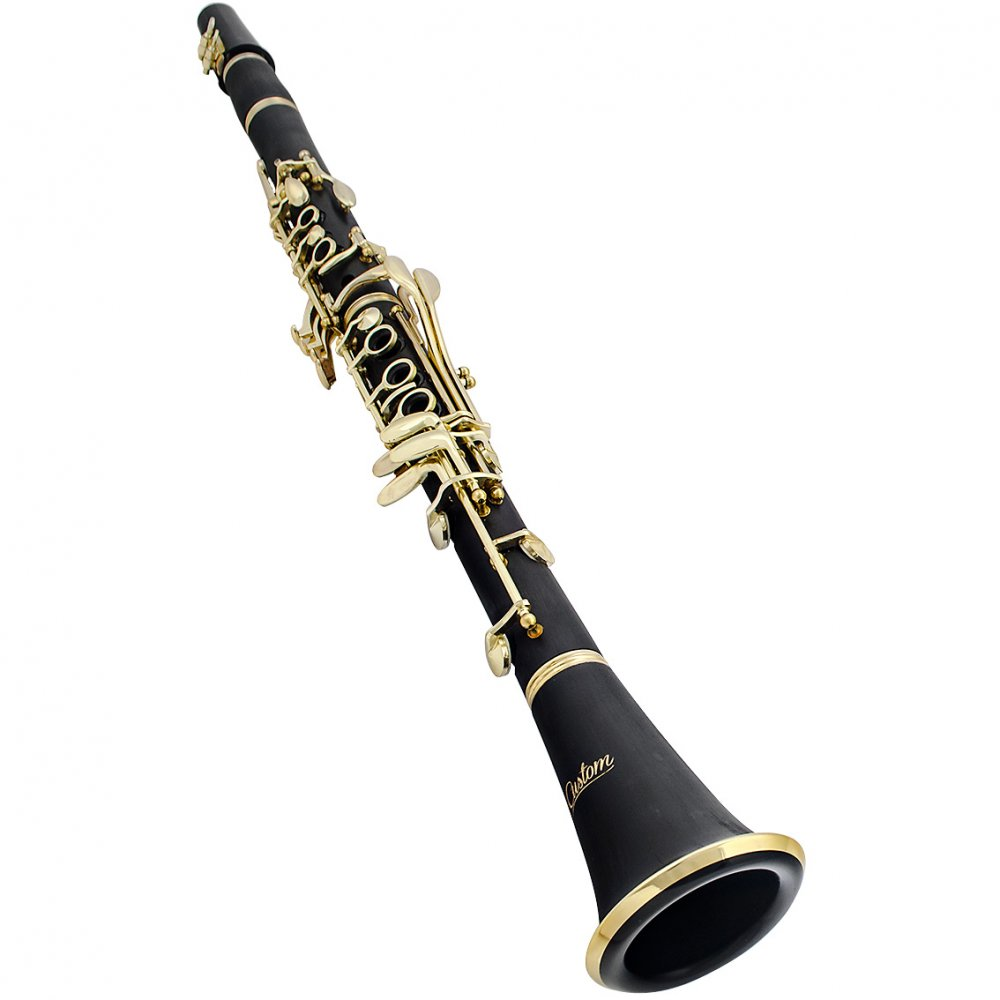
\includegraphics[width=\linewidth/4]{pasta1_figuras/clarinete.jpg}
	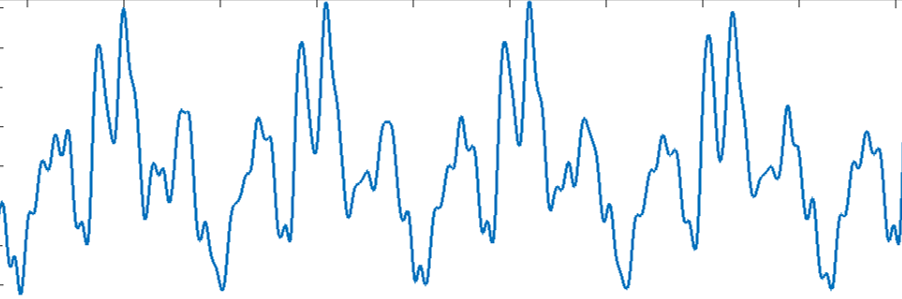
\includegraphics[scale=0.45]{pasta1_figuras/clarinete-timbre.png}
	\caption{Clarinete e sua forma de onda}
	\label{fig-clarinete}
\end{figure}

\subsubsection{Escala: Bb Maior}

O áudio com a escala de Bb Maior no clarinete tem duração de 20 segundos, contando com o tempo inicial sem notas. A Figura \ref{fig-clarinete-escala} exibe a interface gráfica para o experimento com o áudio da escala de Bb Maior.

\begin{figure}
	\centering
	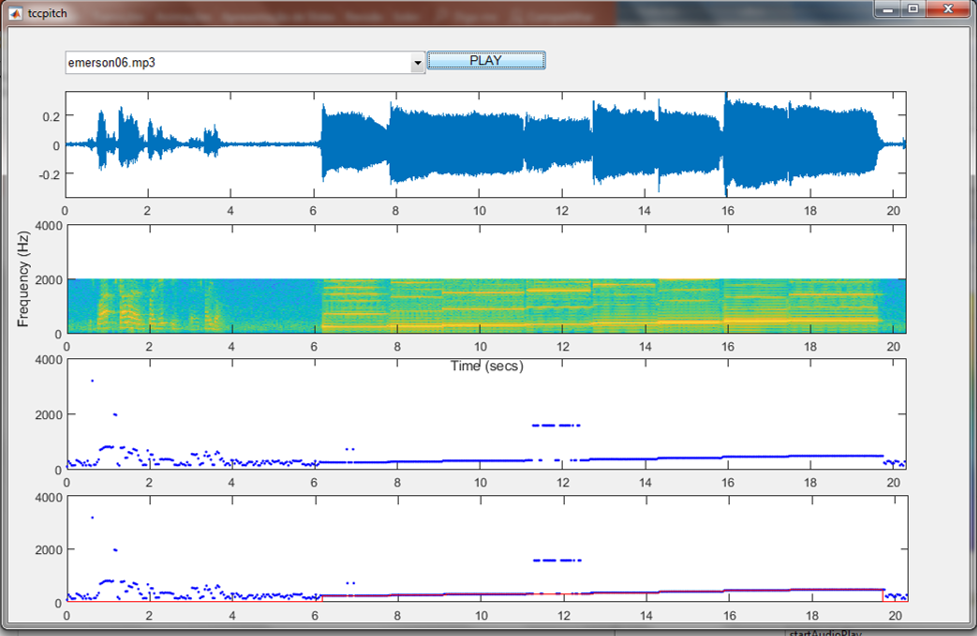
\includegraphics[width=0.75\linewidth]{pasta1_figuras/clarinete-escala.png}
	\caption{Interface de experimentação para áudio "Escala Bb Maior" com clarinete}
	\label{fig-clarinete-escala}
\end{figure}

Os gráficos obtidos no experimento são colocados em separado para melhor visualização das informações. A Figura \ref{fig-clarinete-escala-2} mostra o espectrograma do áudio, a Figura \ref{fig-clarinete-escala-3} exibe as saídas do sistema de detecção de $f_0$, enquanto a Figura \ref{fig-clarinete-escala-4} compara as saídas do sistema de detecção com as frequências esperadas, conforme o arquivo de registros.


Os gráficos demonstram que o sistema obteve sucesso nas detecções de $f_0$, ocorrendo erros em momentos específicos de apenas duas notas, onde detectou-se um harmônico devido ao efeito de ressonância da gravação. Foi calculado um sucesso de 93.4\% nas detecções realizadas para este áudio.

\begin{figure}

\begin{subfigure}{1\textwidth}
	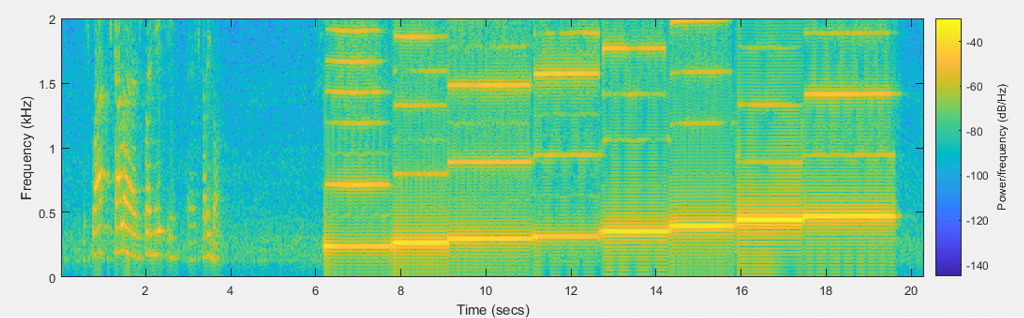
\includegraphics[width=\linewidth]{pasta1_figuras/clarinete-escala-2.png}
	\caption{Espectrograma}
	\label{fig-clarinete-escala-2}
\end{subfigure}
	\hspace*{\fill} % separation between the subfigures
\begin{subfigure}{1\textwidth}
	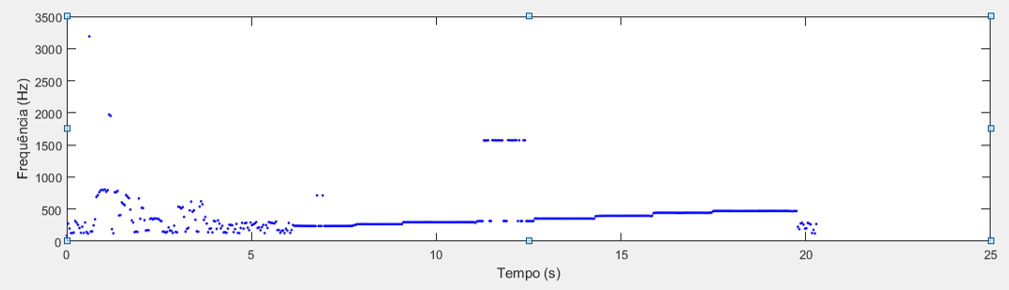
\includegraphics[width=\linewidth]{pasta1_figuras/clarinete-escala-3.png}
	\caption{Detecções de $f_0$}
	\label{fig-clarinete-escala-3}
\end{subfigure}
	\hspace*{\fill} % separation between the subfigures
\begin{subfigure}{1\textwidth}
	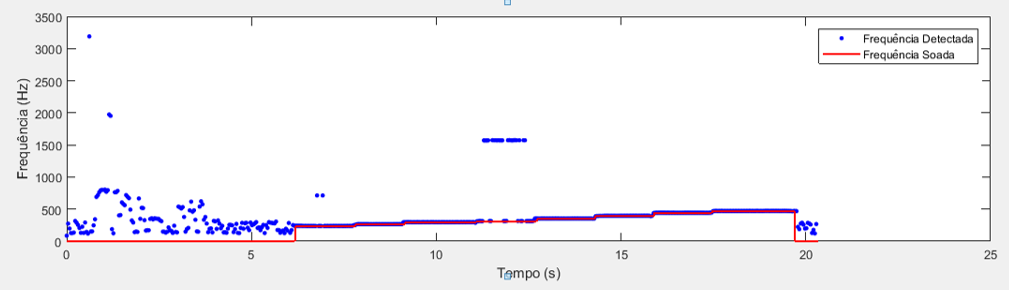
\includegraphics[width=\linewidth]{pasta1_figuras/clarinete-escala-4.png}
	\caption{Comparativo de detecções e registros de $f_0$}
	\label{fig-clarinete-escala-4}
\end{subfigure}
	\caption{Escala de Bb Maior com clarinete}
\end{figure}

\subsubsection{Música: \textit{Agnus Dei}}

O áudio com a música ``\textit{Agnus Dei}'' no clarinete tem duração de 21 segundos. A Figura \ref{fig-clarinete-mario} exibe a interface gráfica para o experimento com esse áudio.

\begin{figure}
	\centering
	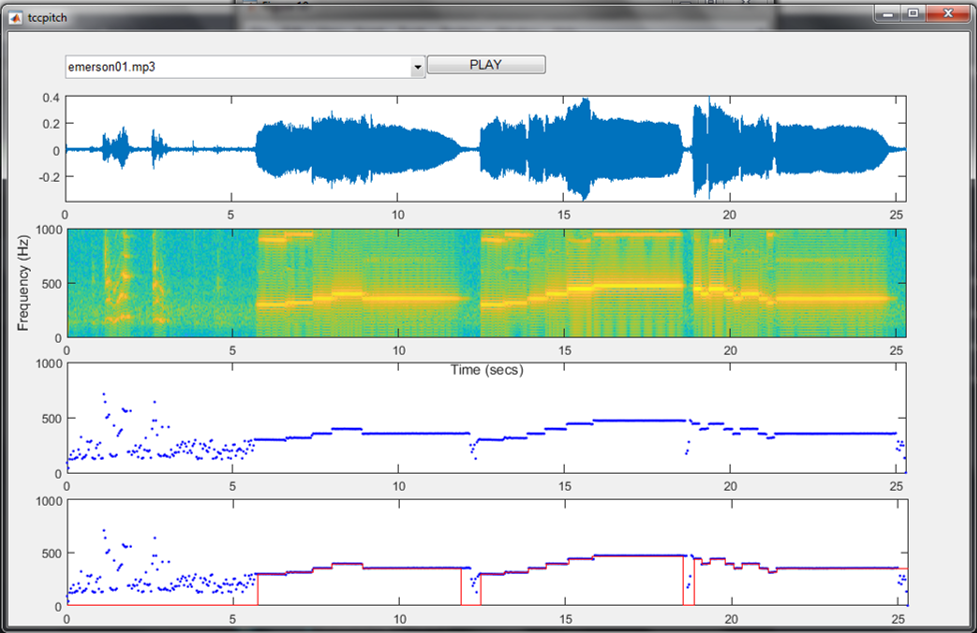
\includegraphics[width=0.75\linewidth]{pasta1_figuras/clarinete-agnusdei.png}
	\caption{Interface de experimentação para áudio da música ``\textit{Agnus Dei}'' com clarinete}
	\label{fig-clarinete-agnusdei}
\end{figure}

Os gráficos obtidos no experimento são colocados em separado para melhor visualização das informações. A Figura \ref{fig-clarinete-mario-2} mostra o espectrograma do áudio, a Figura \ref{fig-clarinete-mario-3} exibe as saídas do sistema de detecção de $f_0$, enquanto a Figura \ref{fig-clarinete-mario-4} compara as saídas do sistema de detecção com as frequências esperadas, conforme o arquivo de registros.


Para esta música, o sistema conseguiu detectar todas as frequências fundamentais, cometendo erro em apenas duas janelas, localizadas em pontos de mudança de nota. O percentual de sucesso na detecção foi de 99.6\%, sendo que os erros podem ser desconsiderados, visto que no instante de alternância entre notas, a janela pode conter mistura de fundamentais da nota anterior com a nova nota que será soada.

\begin{figure}
	\begin{subfigure}{1\textwidth}
		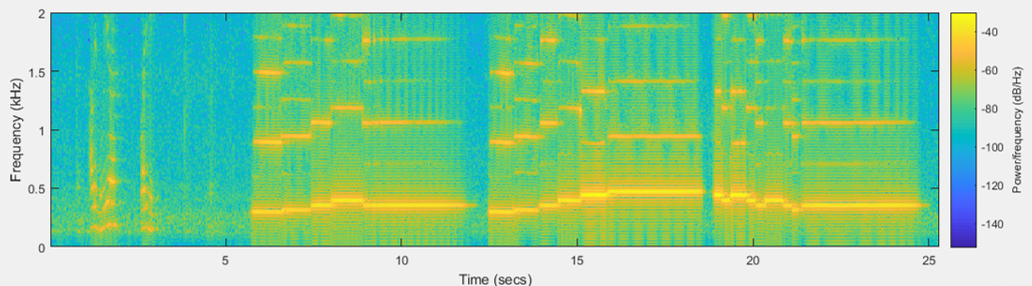
\includegraphics[width=\linewidth]{pasta1_figuras/clarinete-agnusdei-2.png}
		\caption{Espectrograma}
		\label{fig-clarinete-agnusdei-2}
	\end{subfigure}
	\hspace*{\fill} % separation between the subfigures
	\begin{subfigure}{1\textwidth}
		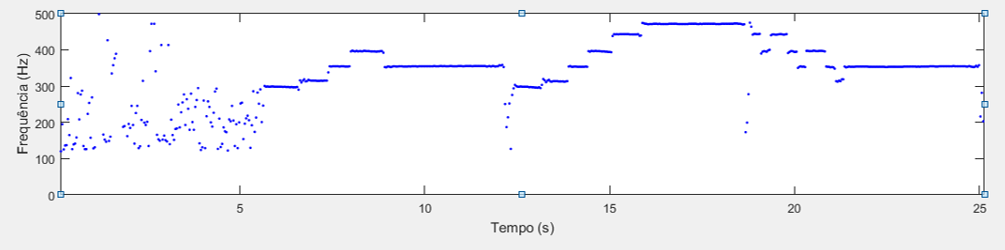
\includegraphics[width=\linewidth]{pasta1_figuras/clarinete-agnusdei-3.png}
		\caption{Detecções de $f_0$}
		\label{fig-clarinete-agnusdei-3}
	\end{subfigure}
	\hspace*{\fill} % separation between the subfigures
	\begin{subfigure}{1\textwidth}
		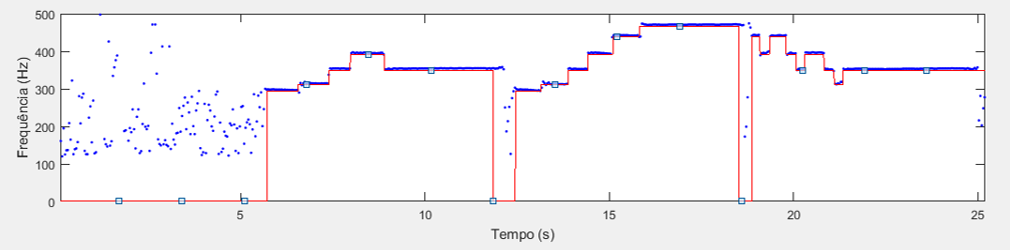
\includegraphics[width=\linewidth]{pasta1_figuras/clarinete-agnusdei-4.png}
		\caption{Comparativo de detecções e registros de $f_0$}
		\label{fig-clarinete-agnusdei-4}
	\end{subfigure}
	\caption{Música ``\textit{Agnus Dei}'' com clarinete}
\end{figure}

\subsubsection{Música: Super Mário Brós}

O áudio com a música tema do \textit{game} ``Super Mário Brós'' no clarinete tem duração de 21 segundos, contando com o tempo inicial sem notas. A Figura \ref{fig-clarinete-mario} exibe a interface gráfica para o experimento com esse áudio.

\begin{figure}
	\centering
	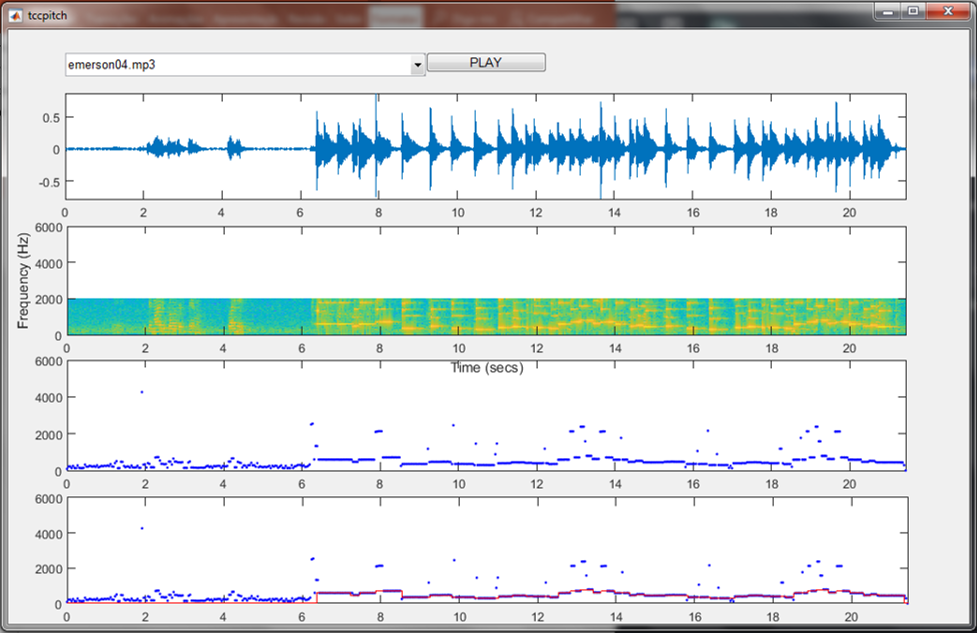
\includegraphics[width=0.75\linewidth]{pasta1_figuras/clarinete-mario.png}
	\caption{Interface de experimentação para áudio da Música ``Super Mário Brós'' com clarinete}
	\label{fig-clarinete-mario}
\end{figure}

Os gráficos obtidos no experimento são colocados em separado para melhor visualização das informações. A Figura \ref{fig-clarinete-mario-2} mostra o espectrograma do áudio, a Figura \ref{fig-clarinete-mario-3} exibe as saídas do sistema de detecção de $f_0$, enquanto a Figura \ref{fig-clarinete-mario-4} compara as saídas do sistema de detecção com as frequências esperadas, conforme o arquivo de registros.


Para este caso, o sistema obteve um bom resultado nas detecções, entretanto, errou em 46 janelas, obtendo um percentual de sucesso nas detecções de 88.2\%. Os erros ocorreram em sua maioria no tempo de subida das notas, e de forma harmônica. Uma característica interessante do clarinete a ser considerada é que, ao soar uma nova nota, se as mãos e a boca do instrumentista não estiverem bem posicionadas no instrumento, percebe-se um leve assobio em um harmônico da nota desejada. Esse efeito ocorre claramente na primeira nota da música tema do ``Super Mário Brós'', e pode ser percebido em mais outra nota durante a execução.

\begin{figure}

\begin{subfigure}{1\textwidth}
	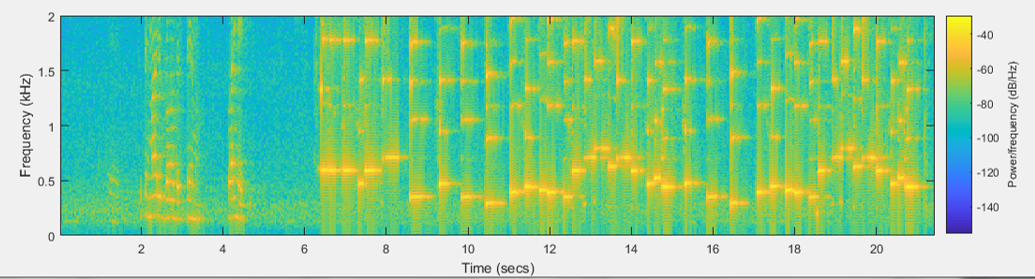
\includegraphics[width=\linewidth]{pasta1_figuras/clarinete-mario-2.png}
	\caption{Espectrograma}
	\label{fig-clarinete-mario-2}
\end{subfigure}

\begin{subfigure}{1\textwidth}
	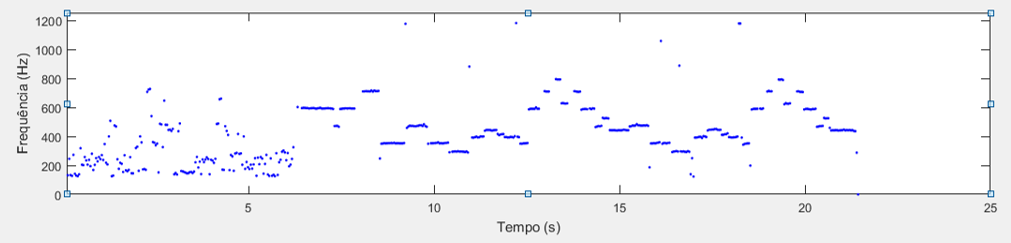
\includegraphics[width=\linewidth]{pasta1_figuras/clarinete-mario-3.png}
	\caption{Detecções de $f_0$}
	\label{fig-clarinete-mario-3}
\end{subfigure}

\begin{subfigure}{1\textwidth}
	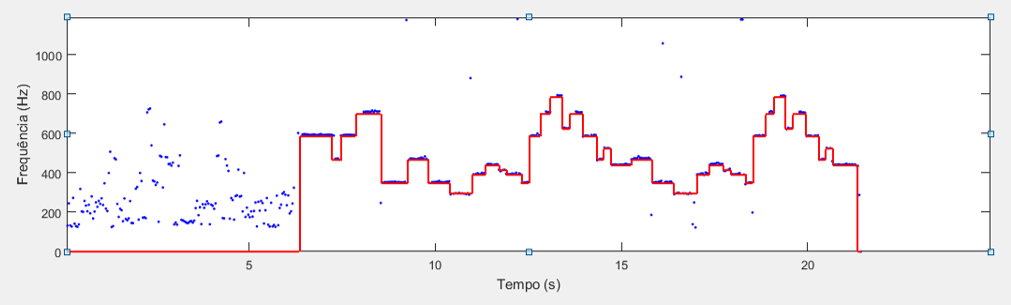
\includegraphics[width=\linewidth]{pasta1_figuras/clarinete-mario-4.png}
	\caption{Comparativo de detecções e registros de $f_0$}
	\label{fig-clarinete-mario-4}
\end{subfigure}
	\caption{Música ``Super Mário Brós'' com clarinete}
\end{figure}



%%%%%
%%
%%
%%%%%

\subsection{Sax Alto}

O Sax Alto também é um instrumento de sopro e, do mesmo modo que o clarinete, está incluso grupo de instrumentos transpositores, ou seja, sua nota soada é diferente da nota escrita na partitura. No caso do sax alto, sua afinação padrão é em Eb. As principais características de seu timbre é o som aveludado, avivado e encorpado. A Figura \ref{fig-sax} mostra o sax alto ao lado de sua forma de onda. Foi realizado experimento com os 3 áudios desse instrumento na base de dados: A escala de Eb, e as músicas ``Deus Cuida de Mim'' e ``\textit{Summertime}''.

\begin{figure}[h!]
	\centering
	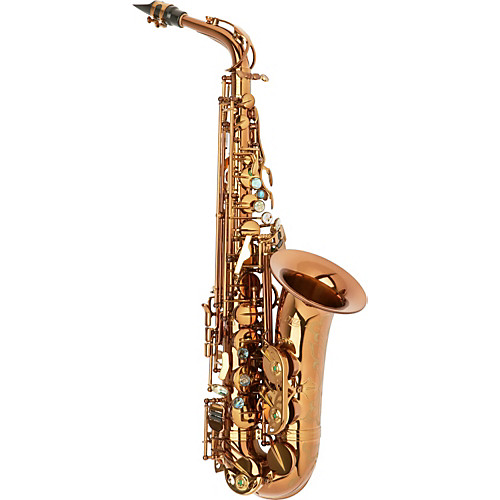
\includegraphics[width=\linewidth/4]{pasta1_figuras/sax.jpg}
	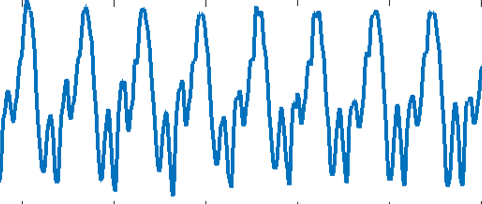
\includegraphics[scale=0.8]{pasta1_figuras/sax-timbre.png}
	\caption{Sax alto e sua forma de onda}
	\label{fig-sax}
\end{figure}

\subsubsection{Escala: Eb Maior}

O áudio com a escala de Eb Maior no sax tem duração de 18 segundos. A Figura \ref{fig-sax-escala} exibe a interface gráfica para o experimento com o áudio da escala de Eb Maior.

\begin{figure}
	\centering
	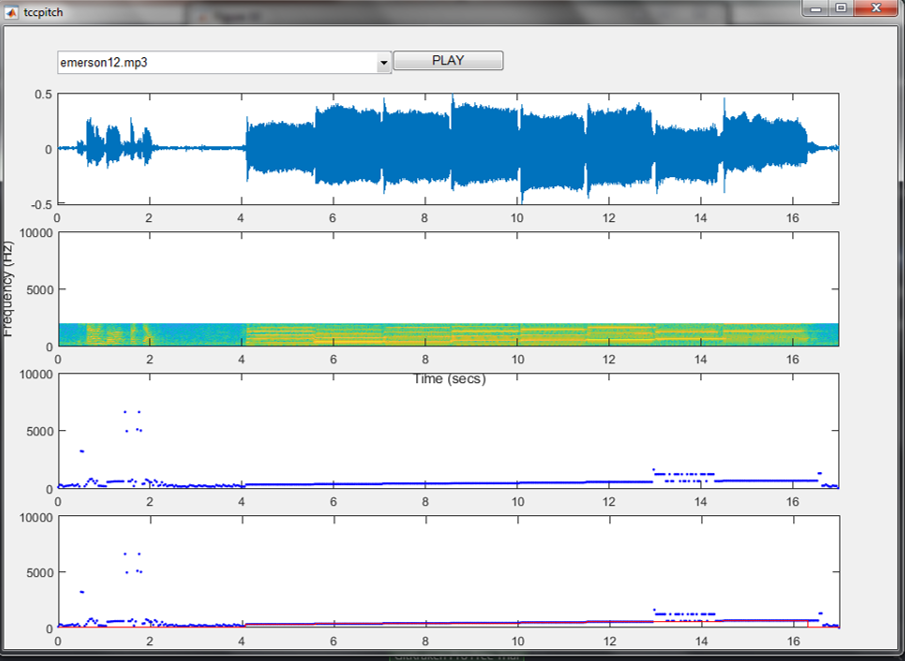
\includegraphics[width=0.75\linewidth]{pasta1_figuras/sax-escala.png}
	\caption{Interface de experimentação para áudio "Escala Eb Maior" com sax alto}
	\label{fig-sax-escala}
\end{figure}

Os gráficos obtidos no experimento são colocados em separado para melhor visualização das informações. A Figura \ref{fig-sax-escala-2} mostra o espectrograma do áudio, a Figura \ref{fig-sax-escala-3} exibe as saídas do sistema de detecção de $f_0$, enquanto a Figura \ref{fig-sax-escala-4} compara as saídas do sistema de detecção com as frequências esperadas, conforme o arquivo de registros.


Para este áudio, o sistema errou a detecção para a nota D5, capturando em mais de 50\% da duração desta nota o harmônico com o dobro da frequência fundamental. Entretanto, não houve nenhum erro nas outras notas. Com isso, o percentual de sucesso na detecção para este áudio foi de 92.8\%, um resultado satisfatório.

\begin{figure}
	
	\begin{subfigure}{1\textwidth}
		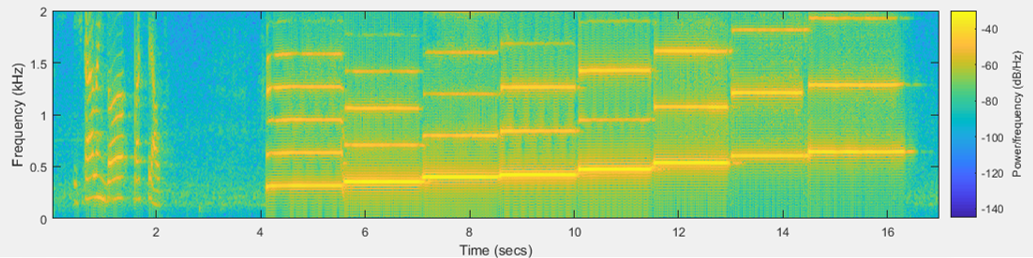
\includegraphics[width=\linewidth]{pasta1_figuras/sax-escala-2.png}
		\caption{Espectrograma}
		\label{fig-sax-escala-2}
	\end{subfigure}
	
	\begin{subfigure}{1\textwidth}
		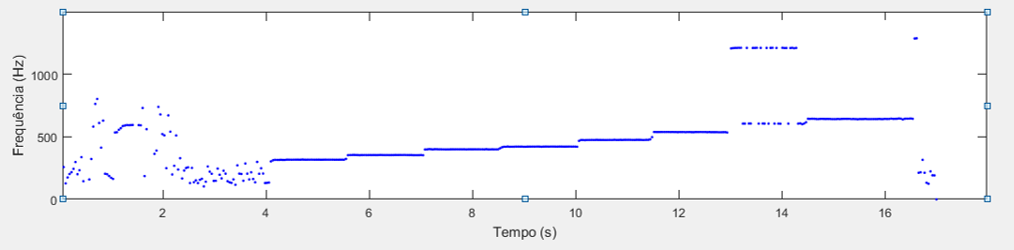
\includegraphics[width=\linewidth]{pasta1_figuras/sax-escala-3.png}
		\caption{Detecções de $f_0$}
		\label{fig-sax-escala-3}
	\end{subfigure}
	
	\begin{subfigure}{1\textwidth}
		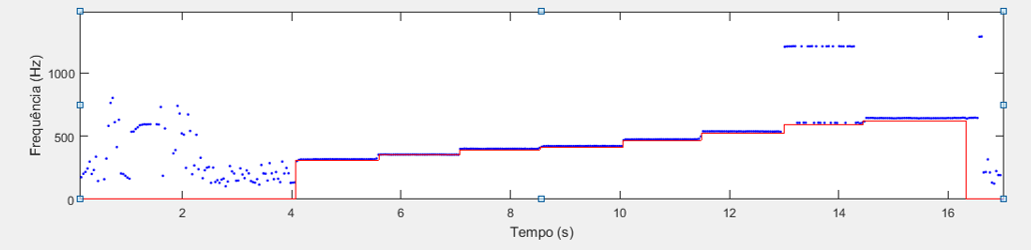
\includegraphics[width=\linewidth]{pasta1_figuras/sax-escala-4.png}
		\caption{Comparativo de detecções e registros de $f_0$}
		\label{fig-sax-escala-4}
	\end{subfigure}
	\caption{Escala Eb Maior com sax alto}
\end{figure}

\subsubsection{Música: Deus Cuida de Mim}

O áudio com a música ``Deus Cuida de Mim'' no sax alto tem duração de 16 segundos. A Figura \ref{fig-sax-Dcm} exibe a interface gráfica para o experimento com esse áudio.

\begin{figure}
	\centering
	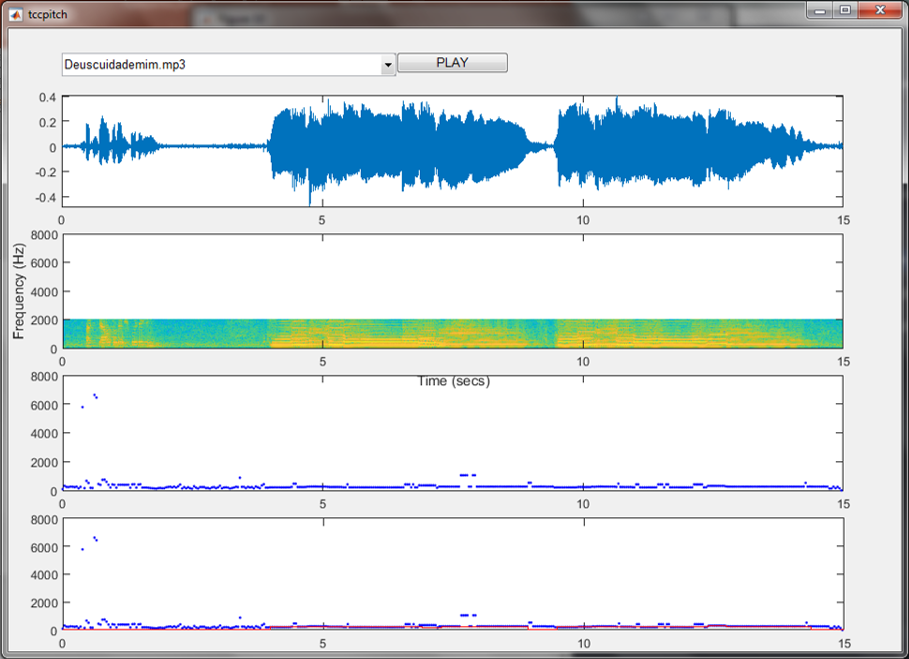
\includegraphics[width=0.75\linewidth]{pasta1_figuras/sax-Dcm.png}
	\caption{Interface de experimentação para áudio da Música ``Deus Cuida de Mim'' com sax alto}
	\label{fig-sax-Dcm}
\end{figure}

Os gráficos obtidos no experimento são colocados em separado para melhor visualização das informações. A Figura \ref{fig-sax-Dcm-2} mostra o espectrograma do áudio, a Figura \ref{fig-sax-Dcm-3} exibe as saídas do sistema de detecção de $f_0$, enquanto a Figura \ref{fig-sax-Dcm-4} compara as saídas do sistema de detecção com as frequências esperadas, conforme o arquivo de registros.


O sistema conseguiu detectar corretamente em 85.9\% das janelas, tendo errado todas as detecções na nota F3. Percebe-se uma real dificuldade em detectar tal nota, pois em ambas as ocorrências dela, detecta-se o harmônico.

\begin{figure}
	
	\begin{subfigure}{1\textwidth}
		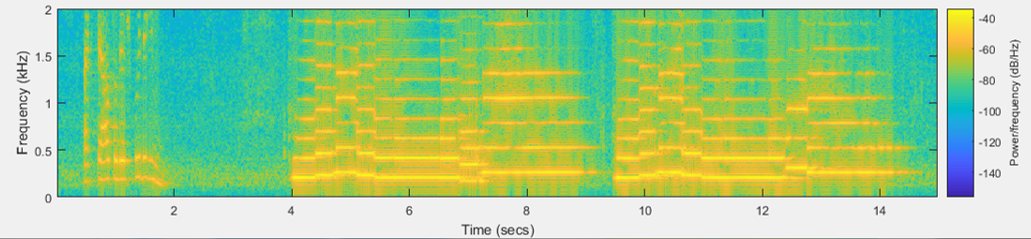
\includegraphics[width=\linewidth]{pasta1_figuras/sax-Dcm-2.png}
		\caption{Espectrograma}
		\label{fig-sax-Dcm-2}
	\end{subfigure}
	\hspace*{\fill} % separation between the subfigures
	\begin{subfigure}{1\textwidth}
		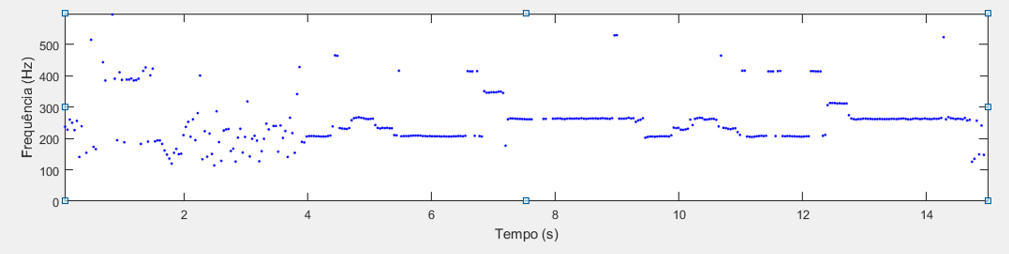
\includegraphics[width=\linewidth]{pasta1_figuras/sax-Dcm-3.png}
		\caption{Detecções de $f_0$}
		\label{fig-sax-Dcm-3}
	\end{subfigure}
	\hspace*{\fill} % separation between the subfigures
	\begin{subfigure}{1\textwidth}
		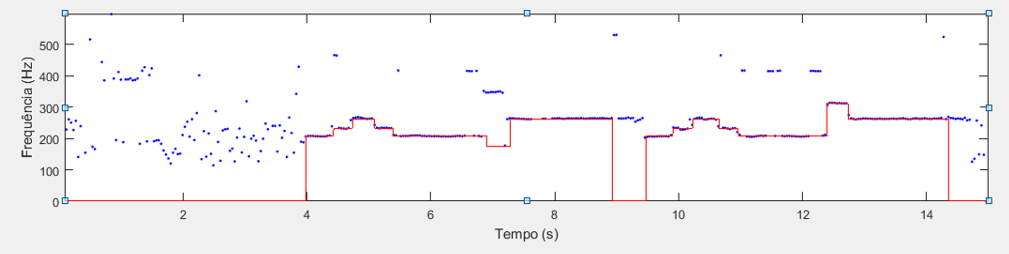
\includegraphics[width=\linewidth]{pasta1_figuras/sax-Dcm-4.png}
		\caption{Comparativo de detecções e registros de $f_0$}
		\label{fig-sax-Dcm-4}
	\end{subfigure}
	\caption{Música ``Deus Cuida de Mim'' no sax alto}
\end{figure}

\subsubsection{Música: \textit{Summertime}}

O áudio com a música ``\textit{Summertime}'' no sax alto tem duração de 29 segundos. A Figura \ref{fig-sax-summer} exibe a interface gráfica para o experimento com esse áudio.

\begin{figure}
	\centering
	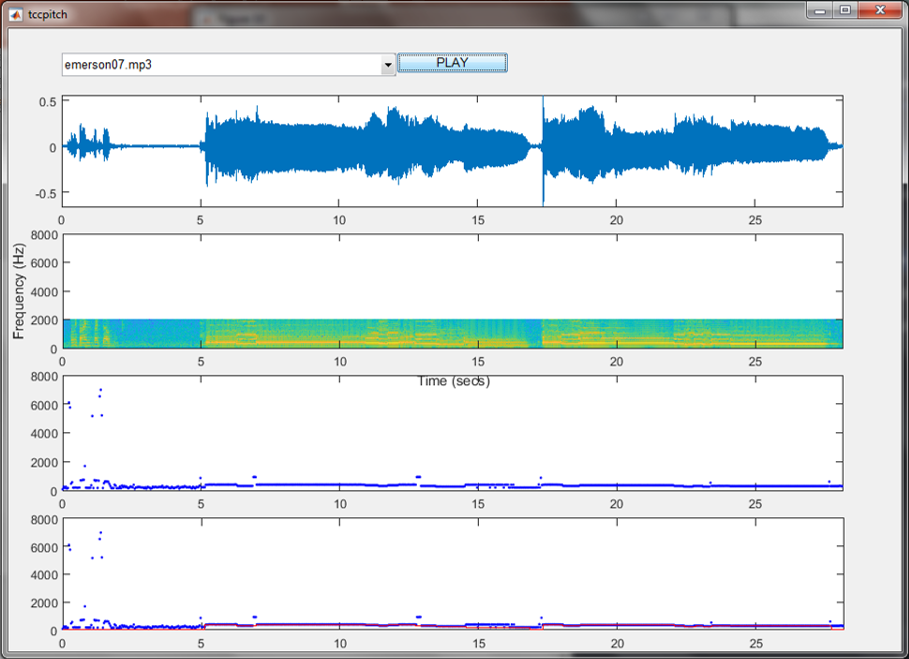
\includegraphics[width=0.75\linewidth]{pasta1_figuras/sax-summer.png}
	\caption{Interface de experimentação para áudio da música ``\textit{Summertime}'' com sax alto}
	\label{fig-sax-summer}
\end{figure}

Os gráficos obtidos no experimento são colocados em separado para melhor visualização das informações. A Figura \ref{fig-sax-summer-2} mostra o espectrograma do áudio, a Figura \ref{fig-sax-summer-3} exibe as saídas do sistema de detecção de $f_0$, enquanto a Figura \ref{fig-sax-summer-4} compara as saídas do sistema de detecção com as frequências esperadas, conforme o arquivo de registros.


Para este áudio, o sistema também errou em mais de 50\% da duração de uma das notas, dessa vez G3, única nota da 3ª escala na música. Entretanto, as detecções nas demais notas, todas da 4ª escala, obtiveram mínimos erros, de modo que a taxa de sucesso nas detecções foi de 91.5\%. Com este áudio, ficou evidente que há uma dificuldade para que o sistema consiga detectar frequências fundamentais para notas abaixo de 200Hz no saxofone alto.


\begin{figure}
	
	\begin{subfigure}{1\textwidth}
		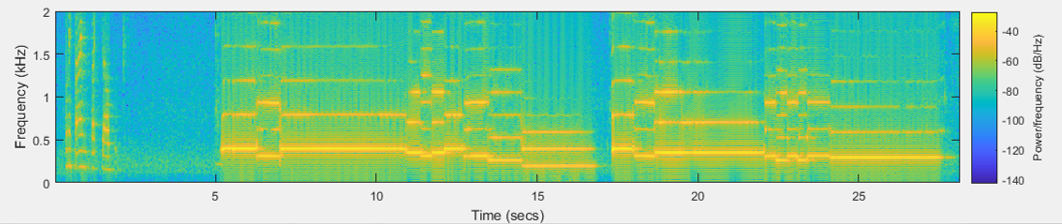
\includegraphics[width=\linewidth]{pasta1_figuras/sax-summer-2.png}
		\caption{Espectrograma}
		\label{fig-sax-summer-2}
	\end{subfigure}
	
	\begin{subfigure}{1\textwidth}
		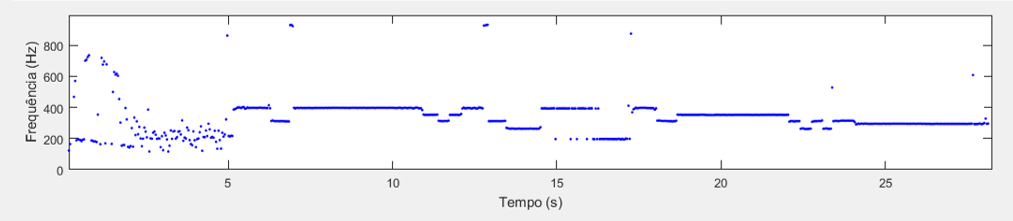
\includegraphics[width=\linewidth]{pasta1_figuras/sax-summer-3.png}
		\caption{Detecções de $f_0$}
		\label{fig-sax-summer-3}
	\end{subfigure}
	
	\begin{subfigure}{1\textwidth}
		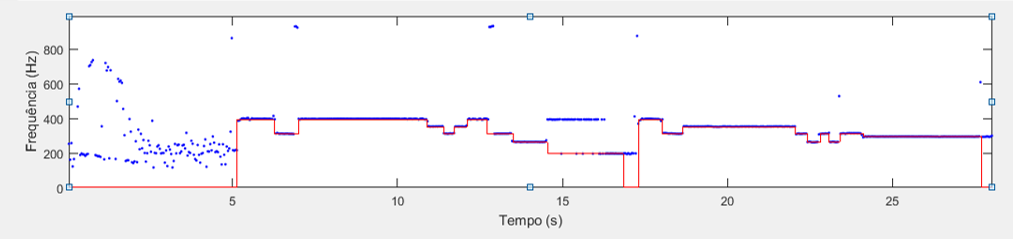
\includegraphics[width=\linewidth]{pasta1_figuras/sax-summer-4.png}
		\caption{Comparativo de detecções e registros de $f_0$}
		\label{fig-sax-summer-4}
	\end{subfigure}
	\caption{Audio da música ``\textit{Summertime}'' no sax alto}
\end{figure}


%%%%%%
%%%
%%%
%%%%%%


\subsection{Piano Eletrônico}

O piano é um instrumento de corda percussivas, entretanto, o piano eletrônico tem o papel de facilitar o uso do piano, de modo que torna-se cada vez mais raro encontrar um piano acústico sendo usado. O piano eletrônico busca imitar o som do piano acústico e, embora não seja perfeitamente igual, já alcança uma boa semelhança. A Figura \ref{fig-piano} mostra o piano eletrônico ao lado de sua forma de onda, responsável pelo timbre do instrumento.

\begin{figure} [h!]
	\centering
	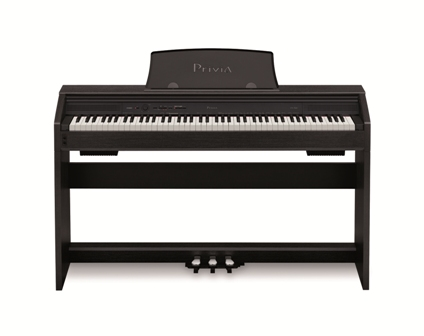
\includegraphics[width=\linewidth/4]{pasta1_figuras/piano.png}
	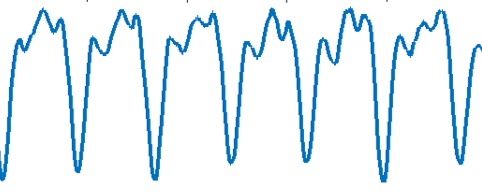
\includegraphics[scale=0.8]{pasta1_figuras/piano-timbre.png}
	\caption{Piano e sua forma de onda}
	\label{fig-piano}
\end{figure}

\subsubsection{Escala: C Maior}

O áudio com a escala de C Maior no piano tem duração de 12 segundos. A Figura \ref{fig-piano-escala} exibe a interface gráfica para o experimento com o áudio da escala de C Maior no piano eletrônico.

\begin{figure}
	\centering
	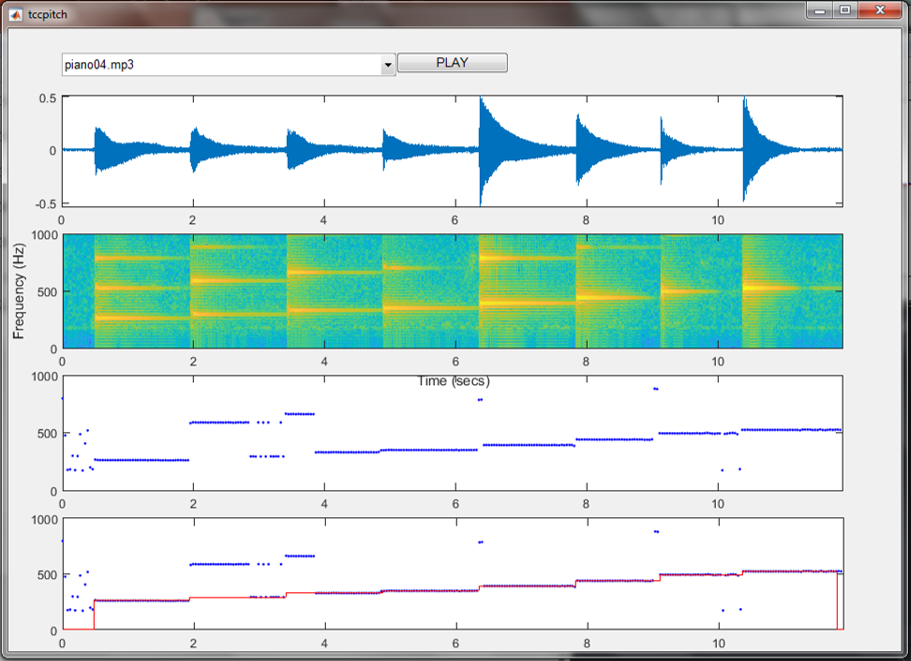
\includegraphics[width=0.75\linewidth]{pasta1_figuras/piano-escala.png}
	\caption{Interface de experimentação para áudio da escala C Maior com piano eletrônico}
	\label{fig-piano-escala}
\end{figure}

Os gráficos obtidos no experimento são colocados em separado para melhor visualização das informações. A Figura \ref{fig-piano-escala-2} mostra o espectrograma do áudio, a Figura \ref{fig-piano-escala-3} exibe as saídas do sistema de detecção de $f_0$, enquanto a Figura \ref{fig-piano-escala-4} compara as saídas do sistema de detecção com as frequências esperadas, conforme o arquivo de registros.


Para a escala de C Maior, o sistema obteve percentual de sucesso nas detecções de 85.1\%. As notas D4 e E4 foram as que mais tiveram erros, tendo suas harmônicas detectadas no dobro da $f_0$ real. Nas demais notas, o sistema conseguiu trabalhar bem.

\begin{figure}
	
	\begin{subfigure}{1\textwidth}
		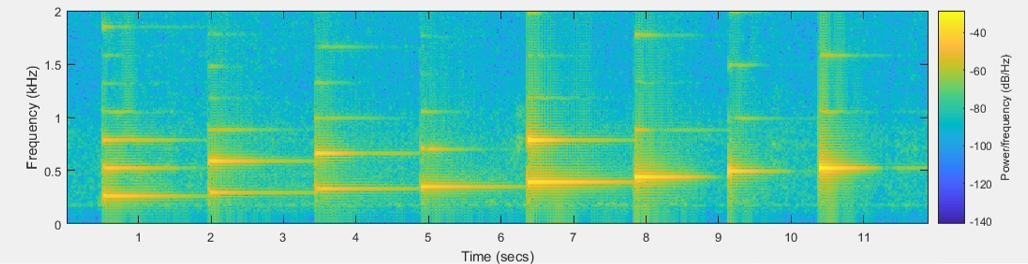
\includegraphics[width=\linewidth]{pasta1_figuras/piano-escala-2.png}
		\caption{Espectrograma}
		\label{fig-piano-escala-2}
	\end{subfigure}
	
	\begin{subfigure}{1\textwidth}
		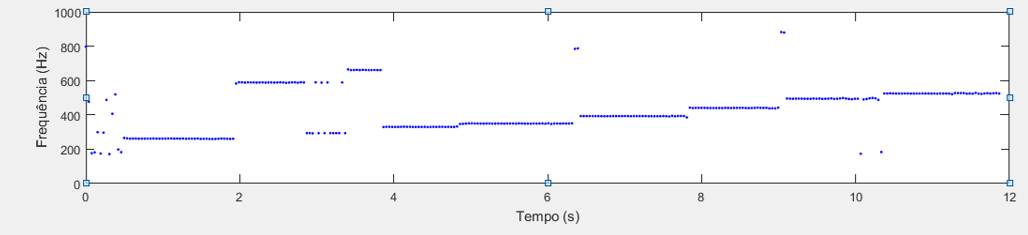
\includegraphics[width=\linewidth]{pasta1_figuras/piano-escala-3.png}
		\caption{Detecções de $f_0$}
		\label{fig-piano-escala-3}
	\end{subfigure}
	
	\begin{subfigure}{1\textwidth}
		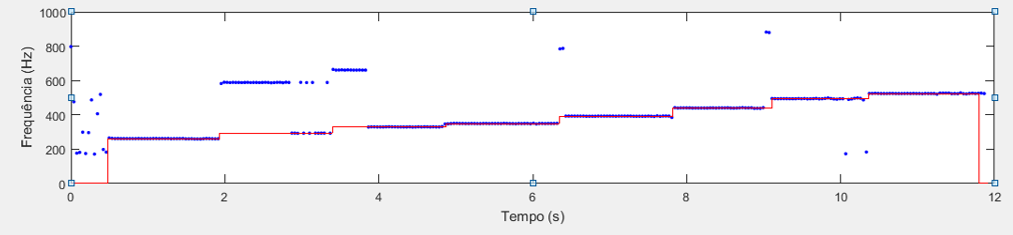
\includegraphics[width=\linewidth]{pasta1_figuras/piano-escala-4.png}
		\caption{Comparativo de detecções e registros de $f_0$}
		\label{fig-piano-escala-4}
	\end{subfigure}
	\caption{Escala de C Maior no piano eletrônico}
\end{figure}

\subsubsection{Música: Eu Navegarei}

O áudio com a música ``Eu Navegarei'' no piano tem duração de 22 segundos. A Figura \ref{fig-piano-navegarei} exibe a interface gráfica para o experimento com esse áudio.

\begin{figure}
	\centering
	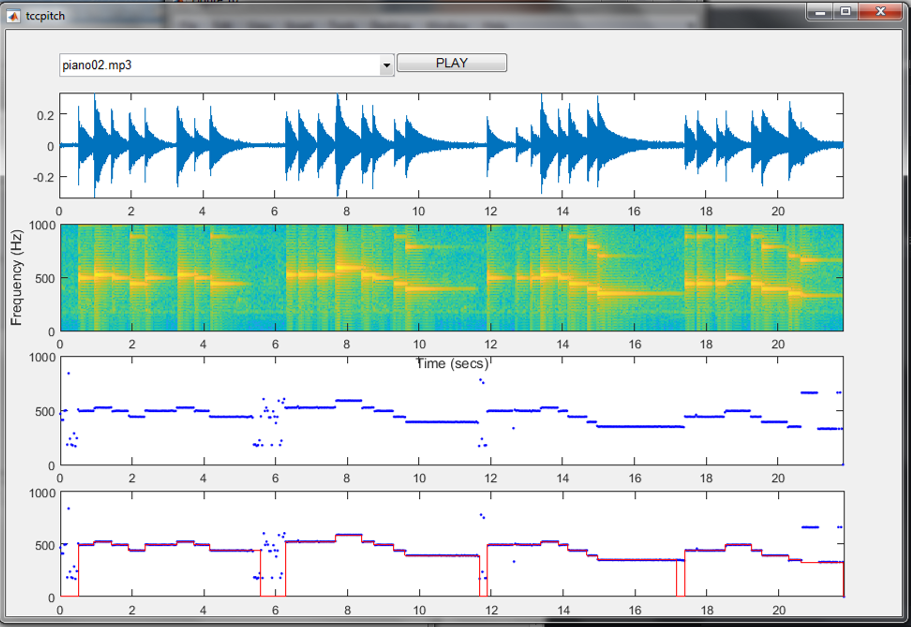
\includegraphics[width=0.75\linewidth]{pasta1_figuras/piano-navegarei.png}
	\caption{Interface de experimentação para áudio da música ``Eu Navegarei'' com piano eletrônico}
	\label{fig-piano-navegarei}
\end{figure}

Os gráficos obtidos no experimento são colocados em separado para melhor visualização das informações. A Figura \ref{fig-piano-navegarei-2} mostra o espectrograma do áudio, a Figura \ref{fig-piano-navegarei-3} exibe as saídas do sistema de detecção de $f_0$, enquanto a Figura \ref{fig-piano-navegarei-4} compara as saídas do sistema de detecção com as frequências esperadas, conforme o arquivo de registros.


Para este áudio, o sistema obteve sucesso em 97\% das janelas analisadas. A maior parte dos 3\% de erros foram durante a execução de uma nota E4, repetindo o problema detectado no áudio da escala de C Maior. Mesmo assim, o sistema alcançou um resultado muito satisfatório para esse experimento

\begin{figure}
	
	\begin{subfigure}{1\textwidth}
		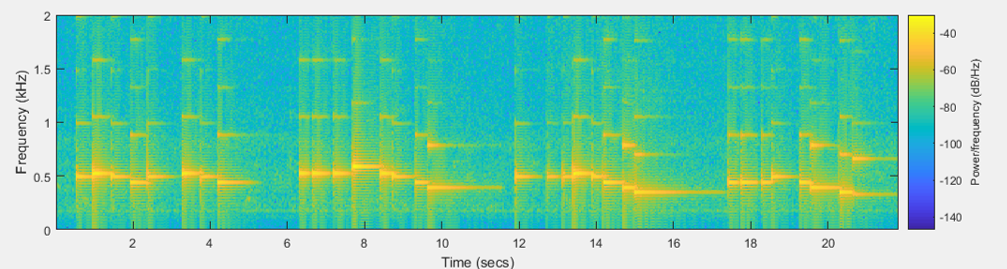
\includegraphics[width=\linewidth]{pasta1_figuras/piano-navegarei-2.png}
		\caption{Espectrograma}
		\label{fig-piano-navegarei-2}
	\end{subfigure}
	\hspace*{\fill} % separation between the subfigures
	\begin{subfigure}{1\textwidth}
		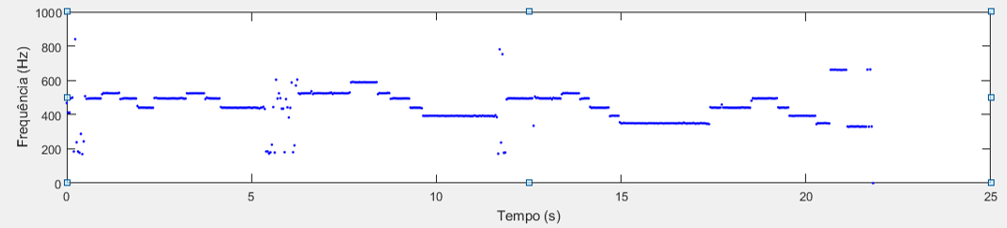
\includegraphics[width=\linewidth]{pasta1_figuras/piano-navegarei-3.png}
		\caption{Detecções de $f_0$}
		\label{fig-piano-navegarei-3}
	\end{subfigure}
	\hspace*{\fill} % separation between the subfigures
	\begin{subfigure}{1\textwidth}
		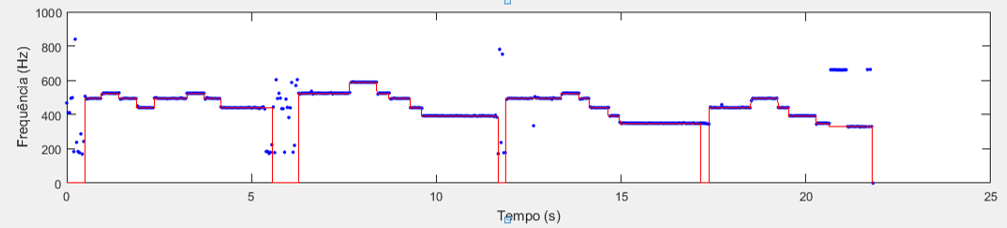
\includegraphics[width=\linewidth]{pasta1_figuras/piano-navegarei-4.png}
		\caption{Comparativo de detecções e registros de $f_0$}
		\label{fig-piano-navegarei-4}
	\end{subfigure}
	\caption{Áudio da música ``Eu Navegarei'' tocado com piano eletrônico}
\end{figure}

\subsubsection{Música: \textit{Skyfall}}

O áudio com a música ``\textit{Skyfall}'' no piano tem duração de 12 segundos. A Figura \ref{fig-piano-skyfall} exibe a interface gráfica para o experimento com esse áudio.

\begin{figure}
	\centering
	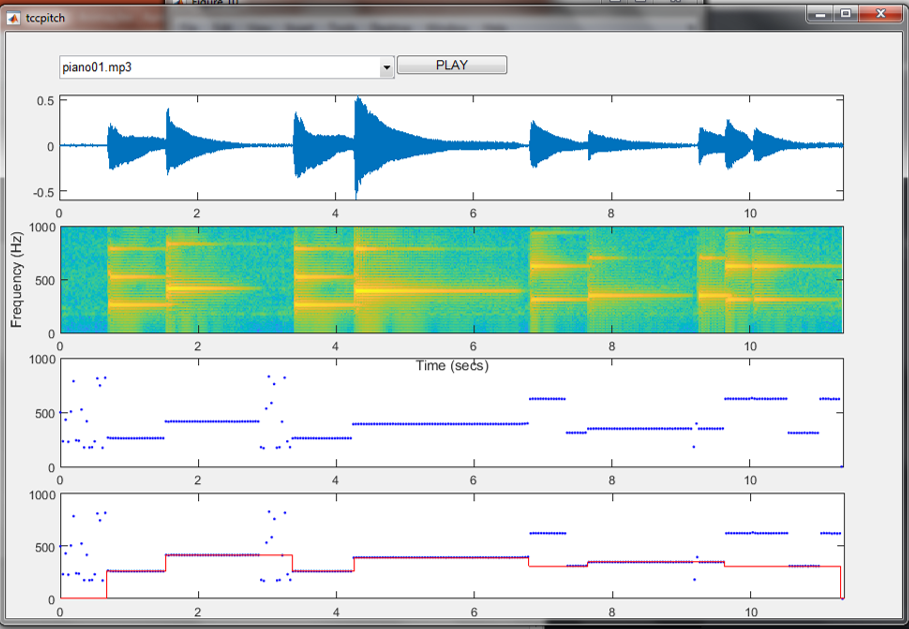
\includegraphics[width=0.75\linewidth]{pasta1_figuras/piano-skyfall.png}
	\caption{Interface de experimentação para áudio da música ``\textit{Skyfall}'' com piano}
	\label{fig-piano-skyfall}
\end{figure}

Os gráficos obtidos no experimento são colocados em separado para melhor visualização das informações. A Figura \ref{fig-piano-skyfall-2} mostra o espectrograma do áudio, a Figura \ref{fig-piano-skyfall-3} exibe as saídas do sistema de detecção de $f_0$, enquanto a Figura \ref{fig-piano-skyfall-4} compara as saídas do sistema de detecção com as frequências esperadas, conforme o arquivo de registros.


Para o áudio ``\textit{Skyfall}'', o sistema teve dois tipos de erros principais: O primeiro refere-se ao problema para detectar Eb4, pois em todos os experimentos com piano eletrônico, o sistema demonstrou uma grande dificuldade em detectar as fundamentais relativas as notas D4, Eb4 e E4, entre 290Hz e 330Hz. O segundo problema esteve relacionado ao  decaimento da nota. Neste áudio, o sistema obteve 79.5\% de taxa de sucesso nas detecções, um valor bem abaixo da média alcançada entre os instrumentos de sopro.

\begin{figure}
	
	\begin{subfigure}{1\textwidth}
		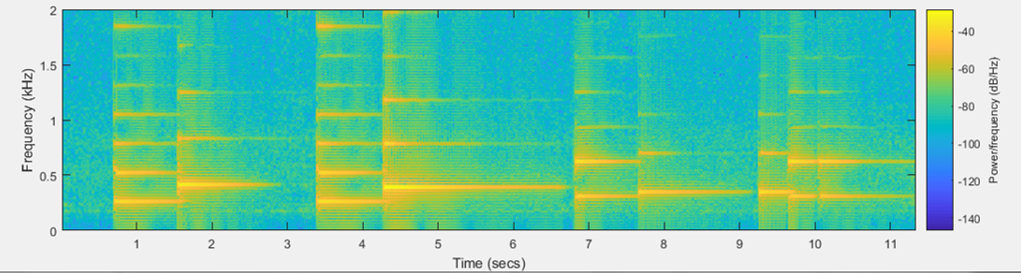
\includegraphics[width=\linewidth]{pasta1_figuras/piano-skyfall-2.png}
		\caption{Espectrograma}
		\label{fig-piano-skyfall-2}
	\end{subfigure}
	
	\begin{subfigure}{1\textwidth}
		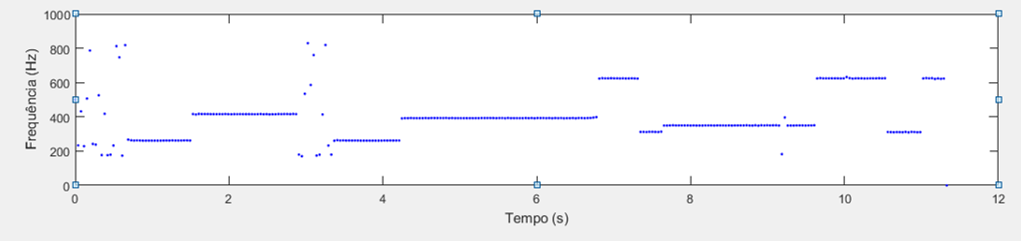
\includegraphics[width=\linewidth]{pasta1_figuras/piano-skyfall-3.png}
		\caption{Detecções de $f_0$}
		\label{fig-piano-skyfall-3}
	\end{subfigure}
	
	\begin{subfigure}{1\textwidth}
		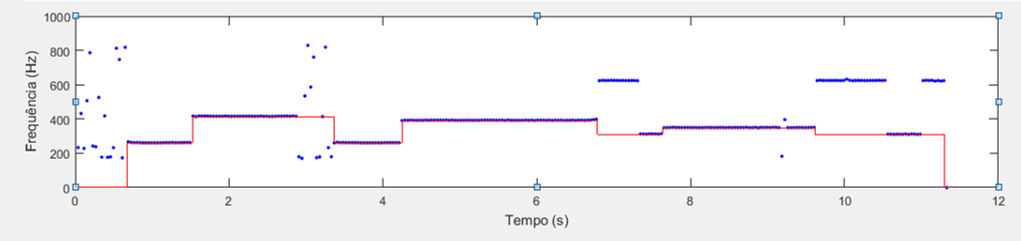
\includegraphics[width=\linewidth]{pasta1_figuras/piano-skyfall-4.png}
		\caption{Comparativo de detecções e registros de $f_0$}
		\label{fig-piano-skyfall-4}
	\end{subfigure}
	\caption{Música ``\textit{Skyfall}'' tocada no piano}
\end{figure}


%%%%%%
%%%
%%%
%%%%%%

\subsection{Violão}

O violão é um instrumento de corda. A Figura \ref{fig-violao} mostra o violão ao lado de sua forma de onda.

\begin{figure}[h!]
	\centering
	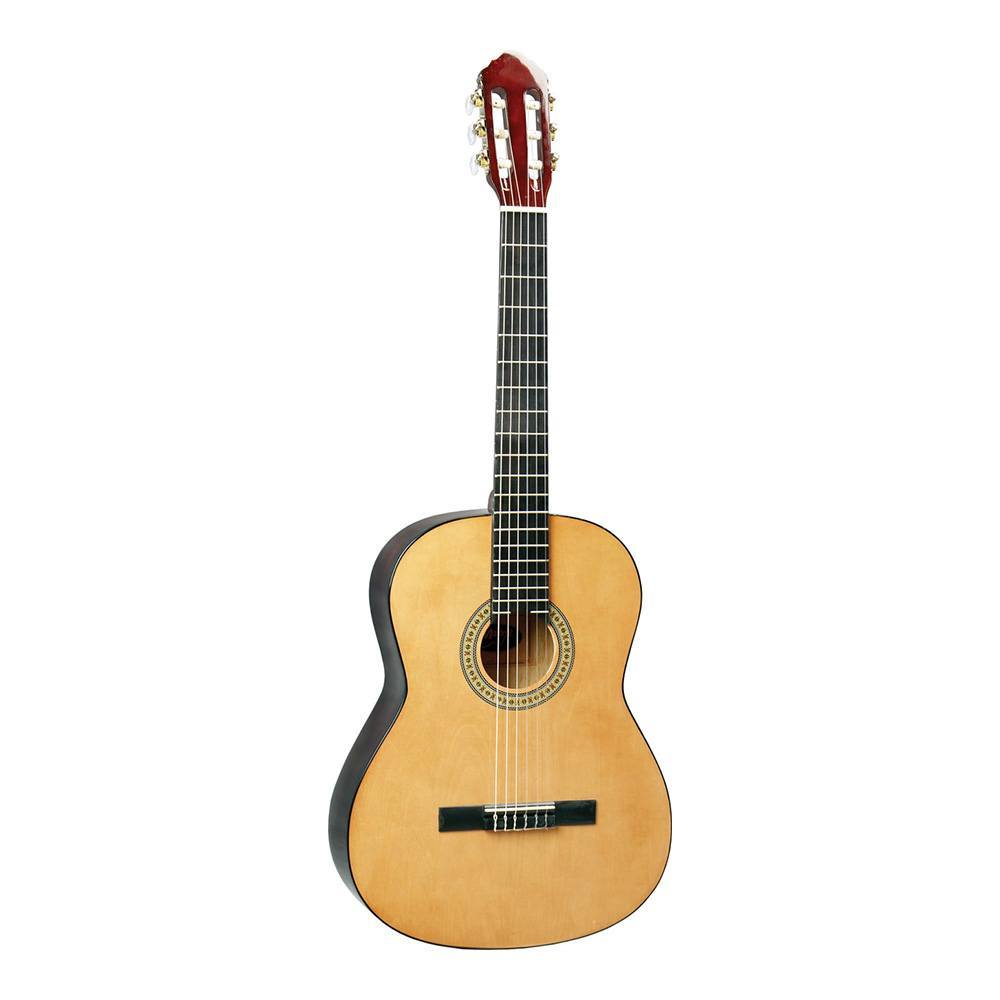
\includegraphics[width=\linewidth/4]{pasta1_figuras/violao.jpg}
	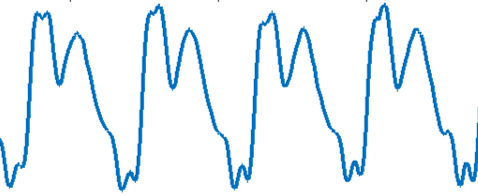
\includegraphics[scale=0.8]{pasta1_figuras/violao-timbre.png}
	\caption{Violão e sua forma de onda}
	\label{fig-violao}
\end{figure}

\subsubsection{Escala: C Maior}

O áudio com a escala de C Maior no violão tem duração de 17 segundos, contando com o tempo inicial de silêncio. A Figura \ref{fig-violao-escala} exibe a interface gráfica para o experimento com o áudio da escala de C Maior tocada pelo violão.

\begin{figure}
	\centering
	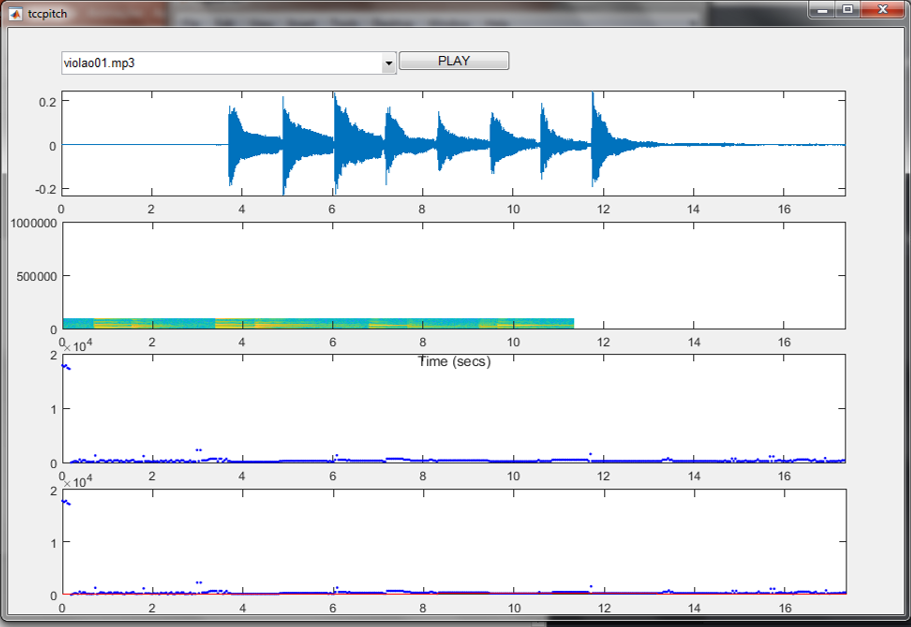
\includegraphics[width=0.75\linewidth]{pasta1_figuras/violao-escala.png}
	\caption{Interface de experimentação para áudio da escala de C Maior com violão}
	\label{fig-violao-escala}
\end{figure}

Os gráficos obtidos no experimento são colocados em separado para melhor visualização das informações. A Figura \ref{fig-violao-escala-2} mostra o espectrograma do áudio, a Figura \ref{fig-violao-escala-3} exibe as saídas do sistema de detecção de $f_0$, enquanto a Figura \ref{fig-violao-escala-4} compara as saídas do sistema de detecção com as frequências esperadas, conforme o arquivo de registros.


Para este áudio, o sistema apresentou o pior resultado, tendo 46.3\% de sucesso nas detecções. Somente as notas C3, A3 e C4 foram detectadas corretamente, enquanto todas as outras foram detectas no harmônico com dobro de $f_0$. A principal característica a ser considerada nessa questão é o funcionamento físico do violão, que amplia o som da vibração de suas cordas através de sua caixa de ressonância. Sendo assim, é comum que o fenômeno da ressonância aconteça, o que atrapalha a performance do sistema. 

\begin{figure}
	
	\begin{subfigure}{1\textwidth}
		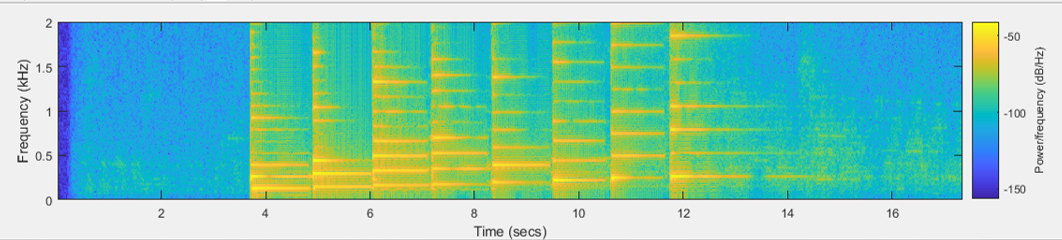
\includegraphics[width=\linewidth]{pasta1_figuras/violao-escala-2.png}
		\caption{Espectrograma}
		\label{fig-violao-escala-2}
	\end{subfigure}
	
	\begin{subfigure}{1\textwidth}
		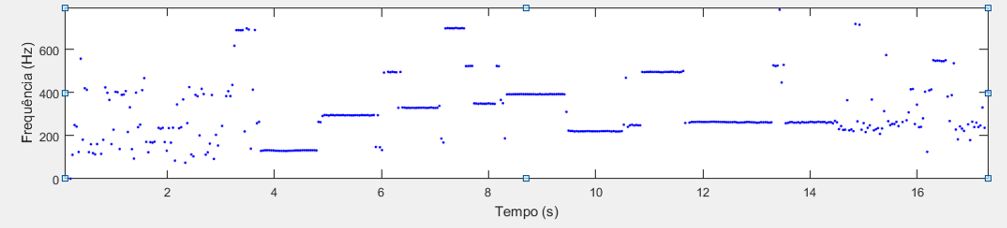
\includegraphics[width=\linewidth]{pasta1_figuras/violao-escala-3.png}
		\caption{Detecções de $f_0$}
		\label{fig-violao-escala-3}
	\end{subfigure}
	
	\begin{subfigure}{1\textwidth}
		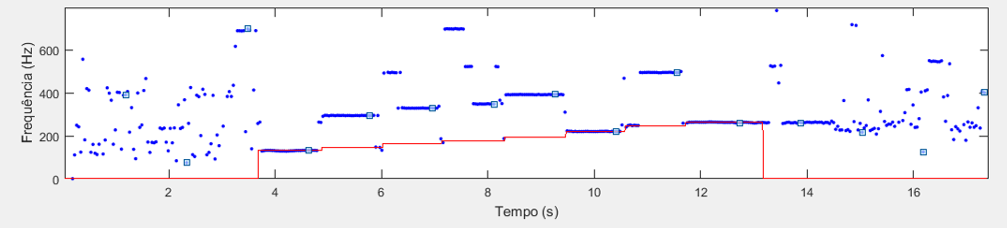
\includegraphics[width=\linewidth]{pasta1_figuras/violao-escala-4.png}
		\caption{Comparativo de detecções e registros de $f_0$}
		\label{fig-violao-escala-4}
	\end{subfigure}
	\caption{Escala de C Maior no violão}
\end{figure}

\subsubsection{Música: Nona Sinfonia}

O áudio com a música ``Nona Sinfonia'' no violão tem duração de 15 segundos, contando com o tempo inicial sem notas. A Figura \ref{fig-violao-nona} exibe a interface gráfica para o experimento com esse áudio.

\begin{figure}
	\centering
	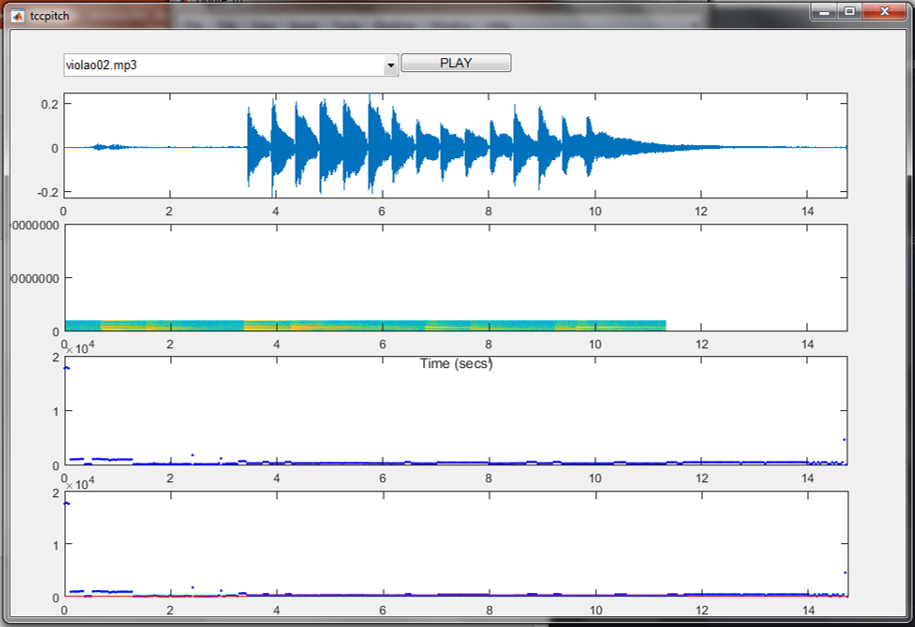
\includegraphics[width=0.75\linewidth]{pasta1_figuras/violao-nona.png}
	\caption{Interface de experimentação para áudio da música ``Nona Sinfonia'' com violão}
	\label{fig-violao-nona}
\end{figure}

Os gráficos obtidos no experimento são colocados em separado para melhor visualização das informações. A Figura \ref{fig-violao-nona-2} mostra o espectrograma do áudio, a Figura \ref{fig-violao-nona-3} exibe as saídas do sistema de detecção de $f_0$, enquanto a Figura \ref{fig-violao-nona-4} compara as saídas do sistema de detecção com as frequências esperadas, conforme o arquivo de registros.


Para este áudio, a detecção obteve taxa de 72.4\% de sucesso nas detecções. Somente a nota G3 que não foi detectada, tendo sido apontado o harmônico da $f_0$. Esse resultado evidencia que a dificuldade com sons mais graves acontece em todos os instrumentos, sendo difícil diferenciar qual o harmônico fundamental.

\begin{figure}
	
	\begin{subfigure}{1\textwidth}
		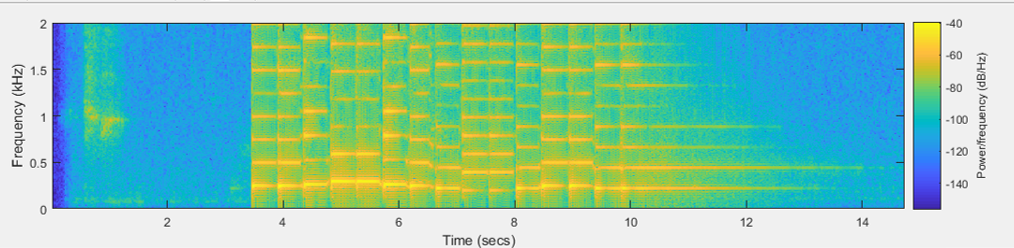
\includegraphics[width=\linewidth]{pasta1_figuras/violao-nona-2.png}
		\caption{Espectrograma}
		\label{fig-violao-nona-2}
	\end{subfigure}
	\hspace*{\fill} % separation between the subfigures
	\begin{subfigure}{1\textwidth}
		\includegraphics[width=\linewidth]{pasta1_figuras/violao-nona-3.png}
		\caption{Detecções de $f_0$}
		\label{fig-violao-nona-3}
	\end{subfigure}
	\hspace*{\fill} % separation between the subfigures
	\begin{subfigure}{1\textwidth}
		\includegraphics[width=\linewidth]{pasta1_figuras/violao-nona-4.png}
		\caption{Comparativo de detecções e registros de $f_0$}
		\label{fig-violao-nona-4}
	\end{subfigure}
		\caption{Música ``Nona Sinfonia'' tocada no violão.}
\end{figure}

\subsubsection{Música: Deus de Abraão}

Por fim, o último áudio a ser analisado foi a música ``Deus de Abraão'' no violão, que tem duração de 22 segundos, contando com o tempo inicial de silêncio. A Figura \ref{fig-violao-002CC} exibe a interface gráfica para o experimento com esse áudio.

\begin{figure}
	\centering
	\includegraphics[width=0.75\linewidth]{pasta1_figuras/violao-002CC.png}
	\caption{Interface de experimentação para áudio da música ``Deus de Abraão'' com violão}
	\label{fig-violao-002CC}
\end{figure}

Os gráficos obtidos no experimento são colocados em separado para melhor visualização das informações. A Figura \ref{fig-violao-002CC-2} mostra o espectrograma do áudio, a Figura \ref{fig-violao-002CC-3} exibe as saídas do sistema de detecção de $f_0$, enquanto a Figura \ref{fig-violao-002CC-4} compara as saídas do sistema de detecção com as frequências esperadas, conforme o arquivo de registros.


Os resultados para esse áudio foram bem acima do esperado, alcançando na detecção de $f_0$, para notas de violão, a taxa de sucesso de 92.6\%. O sucesso se deve principalmente ao uso de notas mais agudas, em maioria da 4ª oitava. Nesse experimento, os erros ocorreram em sua maioria nas 2 notas mais graves, pertencentes a 3ª oitava (F\#3 e B3). Deste modo, fica evidente que o sistema apresenta bons resultados para sons mais agudos, e tem maior dificuldade para discernir sons mais graves.

\begin{figure}
	
	\begin{subfigure}{1\textwidth}
		\includegraphics[width=\linewidth]{pasta1_figuras/violao-002CC-2.png}
		\caption{Espectrograma}
		\label{fig-violao-002CC-2}
	\end{subfigure}
	
	\begin{subfigure}{1\textwidth}
		\includegraphics[width=\linewidth]{pasta1_figuras/violao-002CC-3.png}
		\caption{Detecções de $f_0$}
		\label{fig-violao-002CC-3}
	\end{subfigure}
	
	\begin{subfigure}{1\textwidth}
		\includegraphics[width=\linewidth]{pasta1_figuras/violao-002CC-4.png}
		\caption{Comparativo de detecções e registros de $f_0$}
		\label{fig-violao-002CC-4}
	\end{subfigure}
	\caption{Música ``Deus de Abraão'' tocada no violão.}
\end{figure}



\section{Discussões}

O sistema alcançou resultados satisfatórios, visto que detectou com sucesso um percentual de cerca de 85\% das frequências fundamentais. Entre os instrumentos de sopro, o percentual médio de sucesso ultrapassou os 90\%. Em compensação, percebeu-se que o sistema ainda é deficiente em melodias graves, principalmente para instrumentos de corda. A Tabela \ref{table-compare-songs} exibe as taxas de sucesso obtidas em cada áudio. Os erros nas detecções estiveram em sua maioria relacionados a dificuldade do sistema em detectar fundamentais em notas muito graves, e em outros casos, os erros eram em função de não sustentação da nota ou ruídos de execução. Muitos desses erros podem ser evitados se o sistema for combinado a algum método estatístico de tratamento que identifique a continuidade de uma nota. Entretanto, torna-se um verdadeiro desafio garantir a detecção para notas com efeito de ressonância.

\begin{table}[h]
	\centering
	\caption{Comparativo entre os áudios} 	\label{table-compare-songs}
	\begin{tabular}{|c|c|c|}
		\hline
		\textbf{INSTRUMENTO}       & \textbf{ÁUDIO} & \multicolumn{1}{c|}{\textbf{\begin{tabular}[c]{@{}c@{}}SUCESSO NAS\\ DETECÇÕES\end{tabular}}} \\ \hline
		\multirow{3}{*}{CLARINETE} & Escala - Bb Maior & 93.4\%         \\ \cline{2-3} 
		& Música - \textit{Agnus Dei}  & 99.6\%       \\ \cline{2-3} 
		& Música - Super Mário Brós & 88.2\% \\ \hline
		\multirow{3}{*}{SAX ALTO}  & Escala - Bb Maior  & 92.8\%         \\ \cline{2-3} 
		& Música - Deus Cuida de Mim & 85.9\% \\ \cline{2-3} 
		& Música - \textit{Summertime}   & 91.5\%     \\ \hline
		\multirow{3}{*}{PIANO ELETRÔNICO}     & Escala - C Maior    & 85.1\%       \\ \cline{2-3} 
		& Música - Eu Navegarei   & 97.0\%   \\ \cline{2-3} 
		& Música - \textit{Skyfall}    & 79.5\%     \\ \hline
		\multirow{3}{*}{VIOLÃO}    & Escala - C Maior    & 46.4\%       \\ \cline{2-3} 
		& Música - Nona Sinfonia  & 72.4\%   \\ \cline{2-3} 
		& Música - Ao Deus de Abraão & 92.6\% \\ \hline
	\end{tabular}
\end{table}

O método de detecção de $f_0$ buscando a frequência de maior amplitude, por meio da STFT, é trivialmente falho na ocorrência de ressonância, visto que o efeito de ressonância consiste na superação da amplitude da fundamental por um harmônico em frequência diferente. Diante desse problema, torna-se necessário combinar o método proposto com outros métodos que busquem identificar o efeito de ressonância, de modo a tratar os erros causados por esse efeito. Neste sentido, o sistema implementado apenas da forma como foi proposto não está apto para a detecção de fundamentais em contextos que apresentem o efeito de ressonância. De todo modo, as fundamentais detectadas em 99\% das vezes eram suficientes para fornecer informações da nota soada, divergindo apenas para identificar a oitava a qual essa nota pertence.


A metodologia adotada para a implementação desse projeto mostrou-se de grande potencial, podendo ser evoluída para um sistema mais robusto e com menor sensibilidade ao efeito de ressonância. O ambiente montado para a experimentação também demonstrou ser prático e de fácil manutenção, permitindo que o ritmo de experimentação seja satisfatório. A base de dados foi utilizada com sucesso, e permitiu a verificação de diversos incidentes possíveis na execução de uma melodia no cotidiano do músico, desde os erros humanos até mesmo os efeitos sonoros gerados por cada instrumento, devido às suas particularidades.

% Fim Capítulo